\chapter{Aplicação}

% Referencias - SQLite, JSON, APPCELERATOR TITANIUM, JavaScript, SQL

Tendo como base o questionário apresentado anteriormente onde obtemos maior quantidade de respostas referentes aos acadêmicos de cursos de graduação, foi decidido para este trabalho implementar a aplicação para este público alvo, sendo implementados os módulos que apresentaram as três melhores notas, sendo eles Material de Apoio, Notas da Graduação e Horários do Semestre.

Para o desenvolvimento da aplicação, foi utilizado exclusivamente a ferramenta de desenvolvimento \emph{Titanium SDK} desenvolvida pela \emph{Appcelerator Inc.} devido ao fato de a mesma ser gratuita e utilizar uma linguagem com curva de aprendizado suave. Além disso o fato de utilizar a mesma e desenvolver em JavaScript utilizando ela facilitou a comunicação com o servidor e a extração dos arquivos JSON retornados por ele. Além disso, utilizando-se o \emph{Titanium SDK} para o desenvolvimento, é possível compilar com o mesmo código fonte aplicações para Android e iOS, plataformas mais utilizadas pelos acadêmicos da instituição. Apesar de ser fortemente lembrados os padrões, nem todo o sistema foi desenvolvido utilizando-se os conceitos de orientação a objetos, sendo utilizadas tanto técnicas de programação estruturada como orientação a objetos conforme a técnica que melhor atendia o desenvolvimento do módulo em específico.

Todas as informações extraidas do servidor são inseridas em uma base de dados SQLite no próprio dispositivo, possibilitando assim a consulta offline das informações.

Para facilitar e modularizar este capítulo, as informações referentes a cada módulo foram separadas em sessões que serão apresentadas a seguir.

\section{Base de Dados da Aplicação}

Com o objetivo de armazenar as informações enviadas pelo servidor, foi modelada uma pequena base de dados composta por 5 tabelas utilizadas no armazenamento de dados e uma tabela para armazenamento das configurações. Para esta base de dados foi utilizado o SQLite, nativo nos dispositivos Android e iOS.

\subsection{Tabela de Configuração}
A tabela de configuração é a única tabela não transmitida pelo servidor para a aplicação, sendo gerada e manipulada no próprio dispositivo. A lista de campos e seus respectivos tipos de dados é demonstrada na Tabela 13.

\begin{table}[!hbt]
\centering
\caption[Aplicação - Tabela de Configuração]{Layout da tabela de configuração}
\vspace{3mm}
\begin{tabular}{c|c}\hline
\textbf{Nome do Campo} & \textbf{Tipo de Dados} \\ \hline
login & TEXT \\ \hline
senha & TEXT \\ \hline
\end{tabular}
\\ Fonte: elaboração do autor.
\end{table}

Como pode ser visto, é uma tabela simples que armazena as informações de login, sendo estas utilizadas no para o recebimento das informações atualizadas de dentro do sistema.

\subsection{Tabela de Material de Apoio}
A tabela de Material de apoio é extraida a partir do arquivo JSON de materiais transmitido pelo servidor, e é responsável por armazenar a lista de materiais para todas as disciplinas cursadas pelo acadêmico que está utilizando o aplicativo. Os campos e tipos de dados podem ser consultados na Tabela 14.

\begin{table}[!hbt]
\centering
\caption[Aplicação - Tabela de Material de Apoio]{Layout da tabela de Material de Apoio}
\vspace{3mm}
\begin{tabular}{c|c}\hline
\textbf{Nome do Campo} & \textbf{Tipo de Dados} \\ \hline
nomeDisciplina         & TEXT                   \\ \hline
publicacao             & TEXT                   \\ \hline 
nome                   & TEXT                   \\ \hline
descricao              & TEXT                   \\ \hline
url                    & TEXT                   \\ \hline
\end{tabular}
\\ Fonte: elaboração do autor.
\end{table}

Devido a quantidade de colunas ser reduzida, as informações dos materiais de apoio foi a única que não foi dividida em duas tabelas, sendo possível manter sem problemas as informações em apenas uma tabela, não gerando grande duplicidade nas informações.

\subsection{Tabela de Horários do Semestre}
Com o objetivo de facilitar as consultas SQL executadas na base de dados e fornecer uma complexidade menor na leitura do código, o JSON de Horários do Semestre retornado pelo servidor é extraido em duas tabelas unidas por uma chave. Desta forma, a tabela de Horários do Semestre é responsável pelo armazenamento das disciplinas e seus detalhes. Na Tabela 15 pode-se observar a lista dos campos e seus respectivos tipos.

\begin{table}[!hbt]
\centering
\caption[Aplicação - Tabela de Horários do Semestre]{Layout da tabela de Horários do Semestre}
\vspace{3mm}
\begin{tabular}{c|c}\hline
\textbf{Nome do Campo} & \textbf{Tipo de Dados} \\ \hline
codigo                 & TEXT                   \\ \hline
turma                  & TEXT                   \\ \hline
nome                   & TEXT                   \\ \hline
curso                  & TEXT                   \\ \hline
dataG2                 & TEXT                   \\ \hline
dataG3                 & TEXT                   \\ \hline
professor              & TEXT                   \\ \hline
creditos               & INTEGER                \\ \hline
turno                  & TEXT                   \\ \hline
grade                  & INTEGER                \\ \hline
periodo                & INTEGER                \\ \hline
\end{tabular}
\\ Fonte: elaboração do autor.
\end{table}

\subsection{Tabela de Horários do Semestre por Disciplina}
Responsável por armazenar as informações dos horários das aulas e se as mesmas já ocorreram, esta tabela pode ser considerada uma extenção da tabela de Horários do Semestre, sendo ligada a mesma pelos campos código e turma. Na Tabela 16 são representados todos os campos da tabela e seus respectivos dados.

\begin{table}[!hbt]
\centering
\caption[Aplicação - Tabela de Horários do Semestre por Disciplina]{Layout da tabela de Horários do Semestre por Disciplina}
\vspace{3mm}
\begin{tabular}{c|c}\hline
\textbf{Nome do Campo} & \textbf{Tipo de Dados} \\ \hline
codigo                 & TEXT                   \\ \hline
turma                  & TEXT                   \\ \hline
hora                   & TEXT                   \\ \hline
diasemana              & TEXT                   \\ \hline
data                   & TEXT                   \\ \hline
ocorreu                & TEXT                   \\ \hline
\end{tabular}
\\ Fonte: elaboração do autor.
\end{table}

\subsection{Tabela de Notas da Graduação}
Com o objetivo de facilitar as consultas SQL executadas na base de dados e fornecer uma complexidade menor na leitura do código, o JSON de Notas da Graduação retornado pelo servidor é extraido em duas tabelas unidas por uma chave. Desta forma, a tabela de Notas da Graduação é responsável pelo armazenamento das disciplinas e seus detalhes. Na Tabela 17 pode-se observar a lista dos campos e seus respectivos tipos.

\begin{table}[!hbt]
\centering
\caption[Aplicação - Tabela de Notas da Graduação]{Layout da tabela de Notas da Graduação}
\vspace{3mm}
\begin{tabular}{c|c}\hline
\textbf{Nome do Campo} & \textbf{Tipo de Dados} \\ \hline
nome                   & TEXT                   \\ \hline
notaG1                 & FLOAT                  \\ \hline
notaG3                 & FLOAT                  \\ \hline
notaG2                 & FLOAT                  \\ \hline
mediaFinal             & FLOAT                  \\ \hline
estadoMateria          & TEXT                   \\ \hline
statusAcademico        & TEXT                   \\ \hline
\end{tabular}
\\ Fonte: elaboração do autor.
\end{table}

\subsection{Tabela de Avaliações}
Responsável por armazenar as informações das avaliações já minstradas, esta tabela pode ser considerada uma extenção da tabela de Notas da Graduação, sendo ligada a mesma pelo campo nome. Na Tabela 18 são representados todos os campos da tabela e seus respectivos dados.
    
\begin{table}[!hbt]
\centering
\caption[Aplicação - Tabela de Avaliações]{Layout da tabela de Avaliações}
\vspace{3mm}
\begin{tabular}{c|c}\hline
\textbf{Nome do Campo} & \textbf{Tipo de Dados} \\ \hline
nomeDisciplina         & TEXT                   \\ \hline
peso                   & TEXT                   \\ \hline
nota                   & FLOAT                  \\ \hline
data                   & TEXT                   \\ \hline 
nome                   & TEXT                   \\ \hline
\end{tabular}
\\ Fonte: elaboração do autor.
\end{table}

\section{Conexão ao Servidor e Extração dos Dados}
A conexão com o servidor ocorre conforme explicado no item 5.4 deste trabalho, onde a partir de uma URL utilizando-se de um cliente HTTP para a conexão. Para o sincronismo das aplicações móveis, foi criado um servidor utilizando-se do endereço \url{http://minhaunomovel.no-ip.org}, sendo então necessário utilizar este endereço na montagem da URL de extração das informações. Os passos para conexão e extração dos dados estão representados no \emph{Apêndice B.1}.

O processo de conexão com o servidor e de extração de dados ocorrem em conjunto onde a partir da conexão, caso a informação buscada seja retornada é chamada a função de extração de dados, que efetua a conversão do JSON transmitido pelo servidor em um objeto JavaScript, e posteriormente extrai as informações e insere as mesmas na base de dados. 

Após o recebimento do arquivo JSON referente ao módulo do sistema a ser extraido, o arquivo JSON é convertido para um objeto nativo JavaScript, sendo que sua manipulação se da de forma extremamente simples, onde os vetores anteriormente representados no JSON agora são acessados como vetores da linguagem, e os objetos se tornam objetos realmente, sem necessidade de funções especiais para acessar seus dados. Desta forma, conforme pode ser visto no \emph{Apêndice B.1} as informações preenchidas no objeto JSON são acessadas sem utilização de funções especiais de acesso e inseridas diretamente na base de dados SQLite.

\section{Login e Persistência das Informações}
Sendo o formulário de entrada do sistema, o formulário de login é a ``porta de entrada'' do acadêmico, sendo por meio deste feito a validação dos dados de login, e posteriormente o recebimento das informações. Na Figura 13 pode ser vista a interface deste formulário.

\begin{figure}[!htb]
     \centering
     \caption[Formulário de Login - Interface]{Interface do Formulário de Login}
     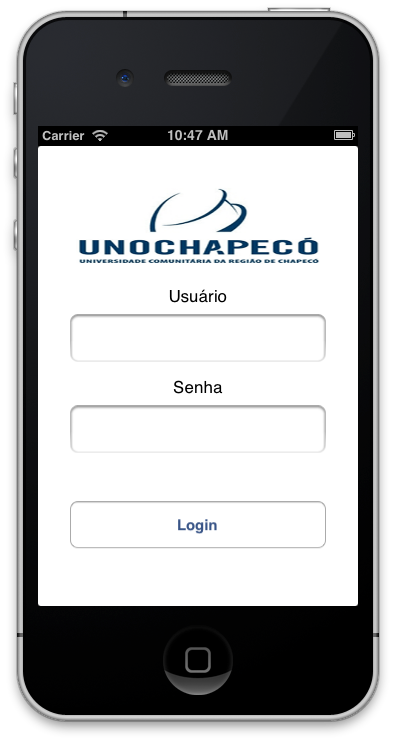
\includegraphics[scale=0.34]{imagens/formlogin.png}
     \\  Fonte: Do Autor.
\end{figure}

Com o objetivo de ser um formulário simples, foi pensado em uma interface limpa, apenas com as informações necessárias. Desta forma o layout a cima foi o escolhido, apenas com os campos de usuário e senha, a logo da instituição e um botão de login.

Após inseridas as informações, no momento que é acionado o botão de login, a aplicação conecta-se com o servidor e recebe os dados do acadêmico. Também neste momento as informações de login e senha são armazenadas na tabela de configuração, sendo que exceto quando o usuário efetua logout (opção sair do menu principal da apliçação), o formulário de login não é mais exibido ao usuário, sendo feito o login de forma automática.

A implementação deste formulário pode ser consultada no \emph{Apêndice B.2}.

\section{Formulário Principal}

Sendo o menu principal da aplicação o formulário principal é a tela de escolha do usuário, onde o mesmo pode acessar os outros menus da aplicação. Seguindo a idéia de simplicidade proposta, utiliza-se de uma lista de opções possuindo acima desta lista a logo da instituição, como pode ser visto na Figura 14.

\begin{figure}[!htb]
     \centering
     \caption[Formulário Principal - Interface]{Interface do Formulário Principal do Aplicativo.}
     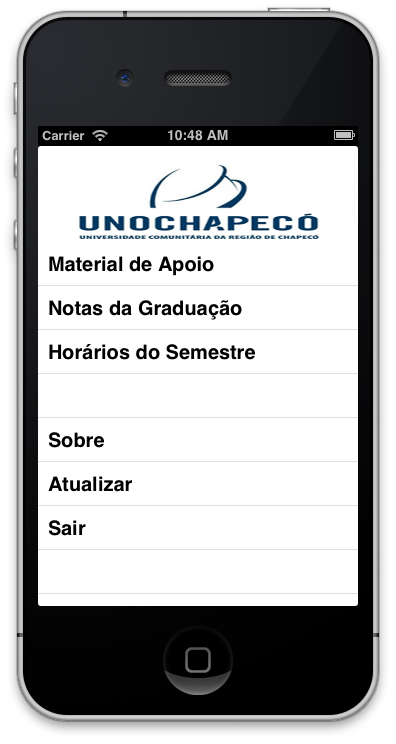
\includegraphics[scale=0.34]{imagens/formprincipal.png}
     \\  Fonte: Do Autor.
\end{figure}

A partir do formulário principal, o usuário pode ser levado para qualquer formulário da aplicação. A opção ``Sobre'' exibe um alerta mostrando mais informações sobre a apliçação, conforme pode ser visto na Figura 15.

\begin{figure}[!htb]
     \centering
     \caption[Formulário Principal - Sobre]{Informações sobre o Aplicativo.}
     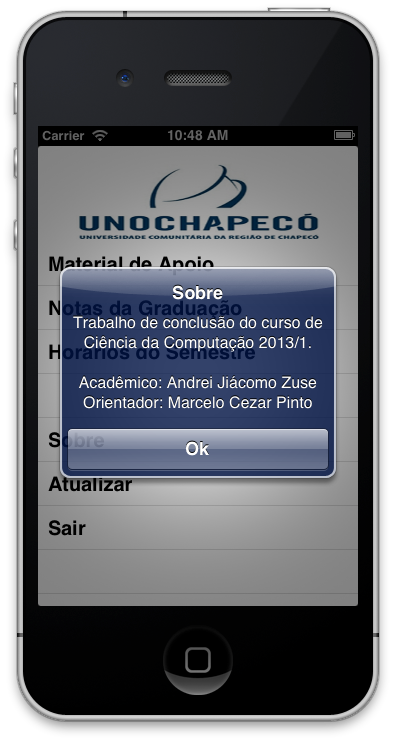
\includegraphics[scale=0.34]{imagens/formsobre.png}
     \\  Fonte: Do Autor.
\end{figure}
\newpage

A opção ``Atualizar'' exibida no menu principal é utilizada pelo usuário para receber novos dados do servidor, sendo assim atualizadas as informações armazenadas no dispositivo. Já a opção ``Sair'' é utilizada para fazer logout do sistema, excluindo as informações armazenadas na base de dados do aplicativo e retornando ao formulário de login.

A implementação deste formulário pode ser consultada no \emph{Apêndice B.3}.


\section{Material de Apoio}
Desenvolvido com o objetivo de permitir a consulta da lista de materiais de apoio das disciplinas, e também permitir visualizar o material (desde que haja suporte pelo dispositivo para visualização do material disponibilizado). Na Figura 16 é possível visualizar o layout da interface gráfica do módulo.

\begin{figure}[!htb]
     \centering
     \caption[Formulário Material de Apoio - Interface]{Interface do Formulário de Material de Apoio.}
     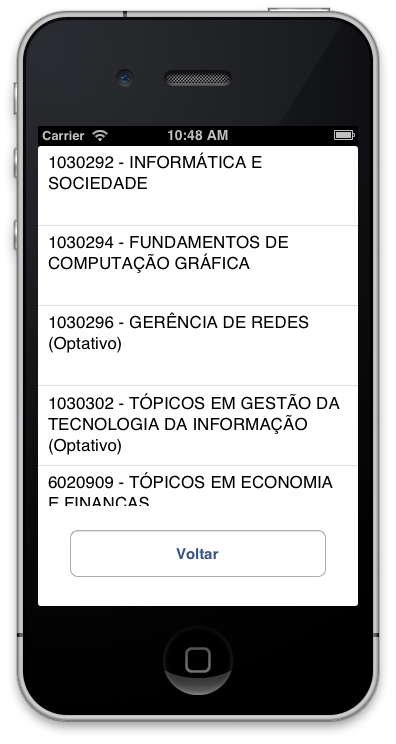
\includegraphics[scale=0.34]{imagens/formmaterialapoio.png}
     \\  Fonte: Do Autor.
\end{figure}

Ao ser selecionada alguma disciplina, a lista dos materiais da mesma é exibida. Para a Figura 17 foi selecionada a disciplina de Informática e Sociedade, carregando assim a lista de materiais da mesma.

\begin{figure}[!htb]
     \centering
     \caption[Formulário Material de Apoio - Consulta de Materiais]{Interface do Formulário de Consulta de Materiais.}
     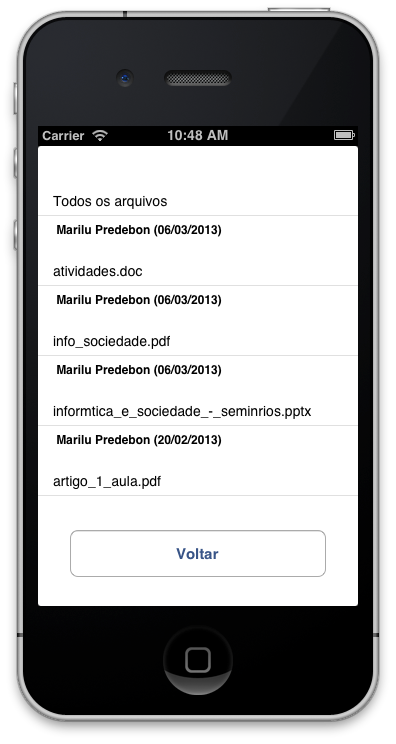
\includegraphics[scale=0.34]{imagens/formmaterialdisciplina.png}
     \\  Fonte: Do Autor.
\end{figure}
\newpage

Ao se escolher uma disciplina, o navegador do dispositivo é chamado, para abrir o material escolhido pelo usuário. Neste ponto é solicitado o login do acadêmico no sistema acadêmico pelo browser, pois não possuímos acesso a sessão em que o arquivo foi extraido no servidor. Após o login, material é exibido, conforme Figura 18.

\begin{figure}[!htb]
     \centering
     \caption[Formulário Material de Apoio - Visualização de Material]{Visualização do Material de Apoio selecionado pelo usuário.}
     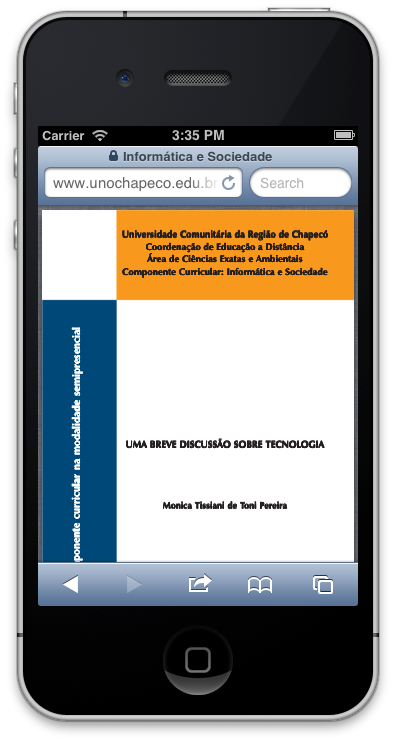
\includegraphics[scale=0.34]{imagens/visualizacaomaterialapoio.png}
     \\  Fonte: Do Autor.
\end{figure}
\newpage

A implementação dos formulários de exibição das disciplinas e dos materiais podem ser consultados nos Apêndices \emph{B.4} e \emph{B.5}.

\section{Notas da Graduação}
O formulário de Notas da Graduação é a interface do usuário para visualização, a partir das disciplinas cursadas pelo mesmo, visualizar suas médias e suas notas por avaliação. Sua interface incial, assim como os outros formulários de consulta, consiste na lista das disciplinas cursadas pelo acadêmico, conforme Figura 19.

\begin{figure}[!htb]
     \centering
     \caption[Formulário Notas da Graduação - Lista das Disciplinas]{Visualização do Formulário de Notas da Graduação.}
     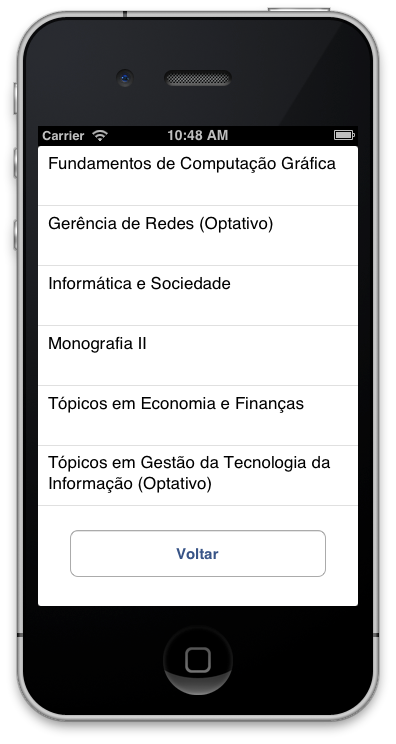
\includegraphics[scale=0.34]{imagens/formnotasgraduacao.png}
     \\  Fonte: Do Autor.
\end{figure}
\newpage

Ao selecionar uma disciplina, é apresentada uma tela com as médias do acadêmico. Caso a disciplina esteja aberta, a tela exibida é semelhante a visualizada na Figura 20. Já caso a disciplina ainda esteja aberta, a imagem exibida é semelhante a Figura 21, exibindo o botão detalhes para a consulta das avaliações feitas pelo acadêmico.

\begin{figure}[!htb]
     \centering
     \caption[Formulário Notas da Graduação - Visualização de Disciplina Fechada]{Visualização das notas de uma disciplina fechada.}
     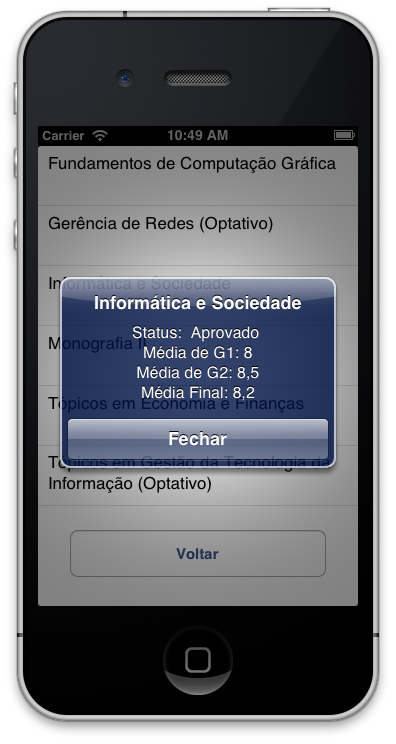
\includegraphics[scale=0.34]{imagens/formvisualizacaomediassemdetalhes.png}
     \\  Fonte: Do Autor.
\end{figure}
\begin{figure}[!htb]
     \centering
     \caption[Formulário Notas da Graduação - Visualização de Disciplina Aberta]{Visualização das notas de uma disciplina em aberto.}
     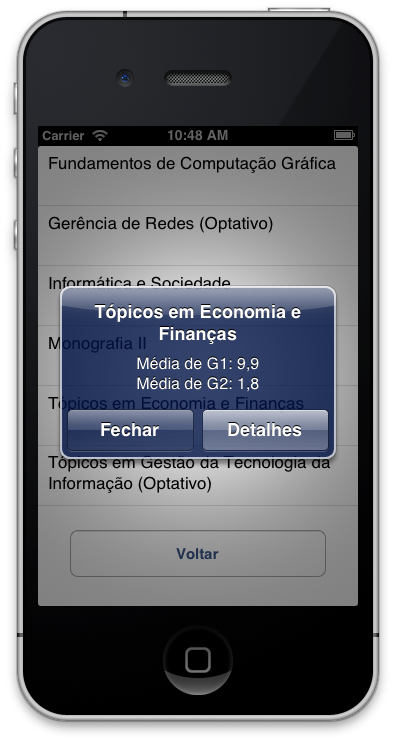
\includegraphics[scale=0.34]{imagens/formvisualizacaomediascomdetalhes.png}
     \\  Fonte: Do Autor.
\end{figure}
\newpage

Em caso de disciplina em aberto, onde o botão ``Detalhes'' é exibido, ao ser escolhio pelo usuário é exibida a tela de avaliações, que mostra as informações referentes as avaliações, caso as mesmas existam (Figura 22), ou é exibida uma mensagem informando que não existem avaliações (Figura 23).

\begin{figure}[!htb]
     \centering
     \caption[Formulário Notas da Graduação - Visualização de Atividades]{Visualização das atividades e suas informações.}
     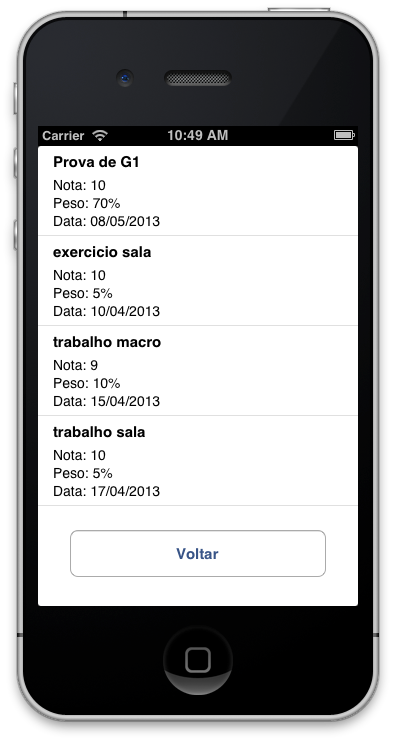
\includegraphics[scale=0.34]{imagens/formatividades.png}
     \\  Fonte: Do Autor.
\end{figure}
\begin{figure}[!htb]
     \centering
     \caption[Formulário Notas da Graduação - Inexistência de Avaliações]{Alerta sobre não existirem avaliações cadastradas no sistema acadêmico.}
     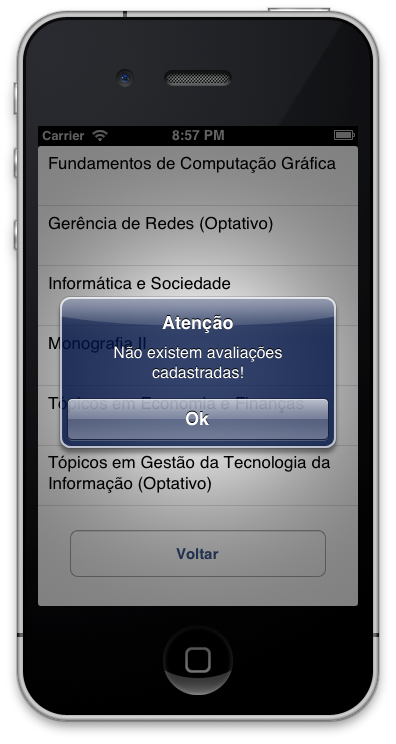
\includegraphics[scale=0.34]{imagens/alertanaoexistemavaliacoes.png}
     \\  Fonte: Do Autor.
\end{figure}

A implementação dos formulários de exibição das disciplinas e das avaliações podem ser consultados nos Apêndices \emph{B.6} e \emph{B.7}.

\section{Horários do Semestre}
O formulário de horários do semestre exibe tanto informações detalhadas sobre a disciplina cursada pelo acadêmico como também os dias de aula da disciplina. Ao ser acessado, assim como os outros formulários, é exibida a lista das disciplinas cursadas, conforme mostrado na Figura 24.
\begin{figure}[!htb]
     \centering
     \caption[Formulário Horários do Semestre - Lista das Disciplinas]{Visualização do Formulário de Horários do Semestre.}
     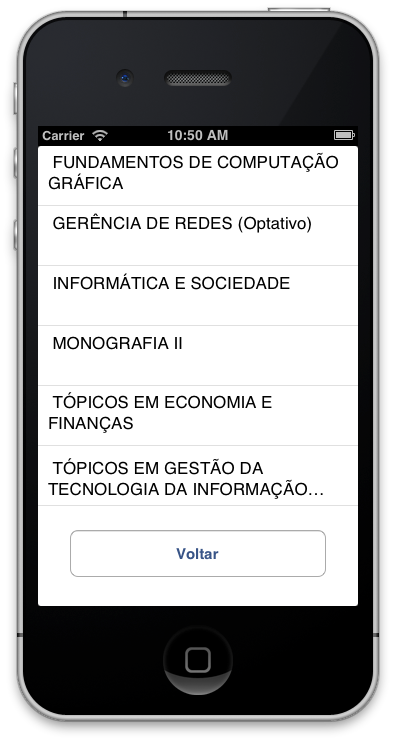
\includegraphics[scale=0.34]{imagens/formhorariosemestre.png}
     \\  Fonte: Do Autor.
\end{figure}

Ao selecionar uma disciplina na lista apresentada, é exibido ao acadêmico um alerta com as informações da disciplina (Figura 25) e também um botão detalhes, que exibe a lista completa de datas e horários de aula da disciplina escolhida (Figura 26).

\begin{figure}[!htb]
     \centering
     \caption[Formulário Horários do Semestre - Visualização de Informações]{Visualização dos detalhes da disciplina selecionada.}
     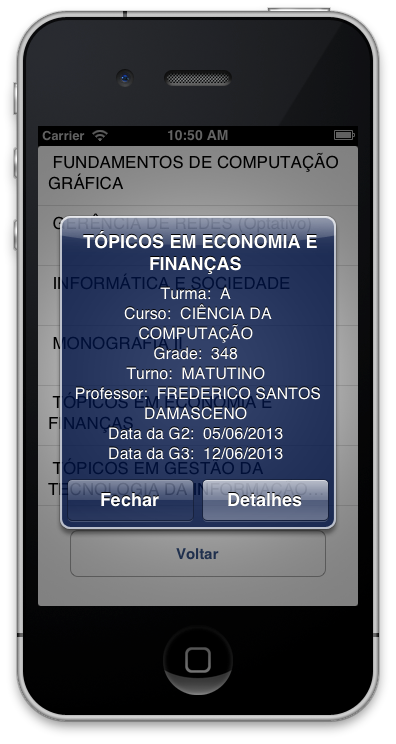
\includegraphics[scale=0.34]{imagens/formhorariossemestredetalhes.png}
     \\  Fonte: Do Autor.
\end{figure}
\begin{figure}[!htb]
     \centering
     \caption[Formulário Horários do Semestre - Visualização dos Horários]{Visualização das datas e horários de aula.}
     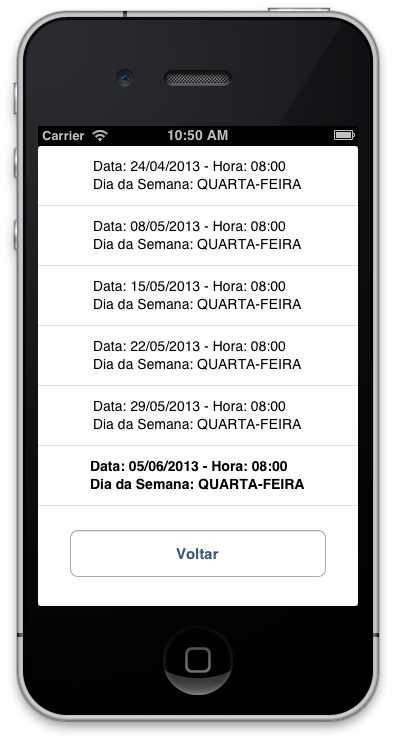
\includegraphics[scale=0.34]{imagens/formconsultahorariosemestredisciplina.png}
     \\  Fonte: Do Autor.
\end{figure}
\newpage

Conforme pode ser visto na Figura 26, o último registro é exibido em destaque. Isto significa que a aquela aula ainda não foi realizada, assim como ocorre no sistema acadêmico Minha Uno.

A implementação dos formulários de exibição das disciplinas e dos horários podem ser consultados nos Apêndices \emph{B.8} e \emph{B.9}.

\section{Execução no Google Android}
